\subsection{Frequency Inverter Analog Input Test}\label{ssec:frequency-inverter-analog-input-test}
	
	\subsubsection{Analog Output Duty Cycle Tests}\label{sec:duty-cycle-test}

		In order to test the analog output of the system an additional test using just a serial terminal was performed to validade the analog output and its usage with the frequency inverter. Before starting this test the frequency inverter was configured to take the 0-10V analog input as its speed reference with a gain of two and maximum rotation of 500rpm. Whereas, when 5V is present at this analog input the rotor should spin at a rotation close to 500rpm and when 2.5V is present at the input the rotor should spin at a rotation close to 250rpm.
		\par
		The test was carried out varying the analog output from 50 to 100$\%$ duty cycle (2.5 to 5V), taking 50 samples at every 10$\%$ interval, \textit{i.e.} taking 50 samples at 50$\%$, 50 samples at 60$\%$, 50 samples at 70$\%$, 50 samples at 80$\%$, 50 samples at 90$\%$ and finally 50 samples at 100$\%$. At each sample the CKP acquisition channel and the analog output feedback channel were monitored.
	
	\subsubsection{Results and Discussion}\label{sec:duty-cycle-test-results}
		Figure \ref{fig:test-analog-voltage} shows the analog output voltage in respect with the duty cycle.

		\begin{figure}[htbp]
				\centering
				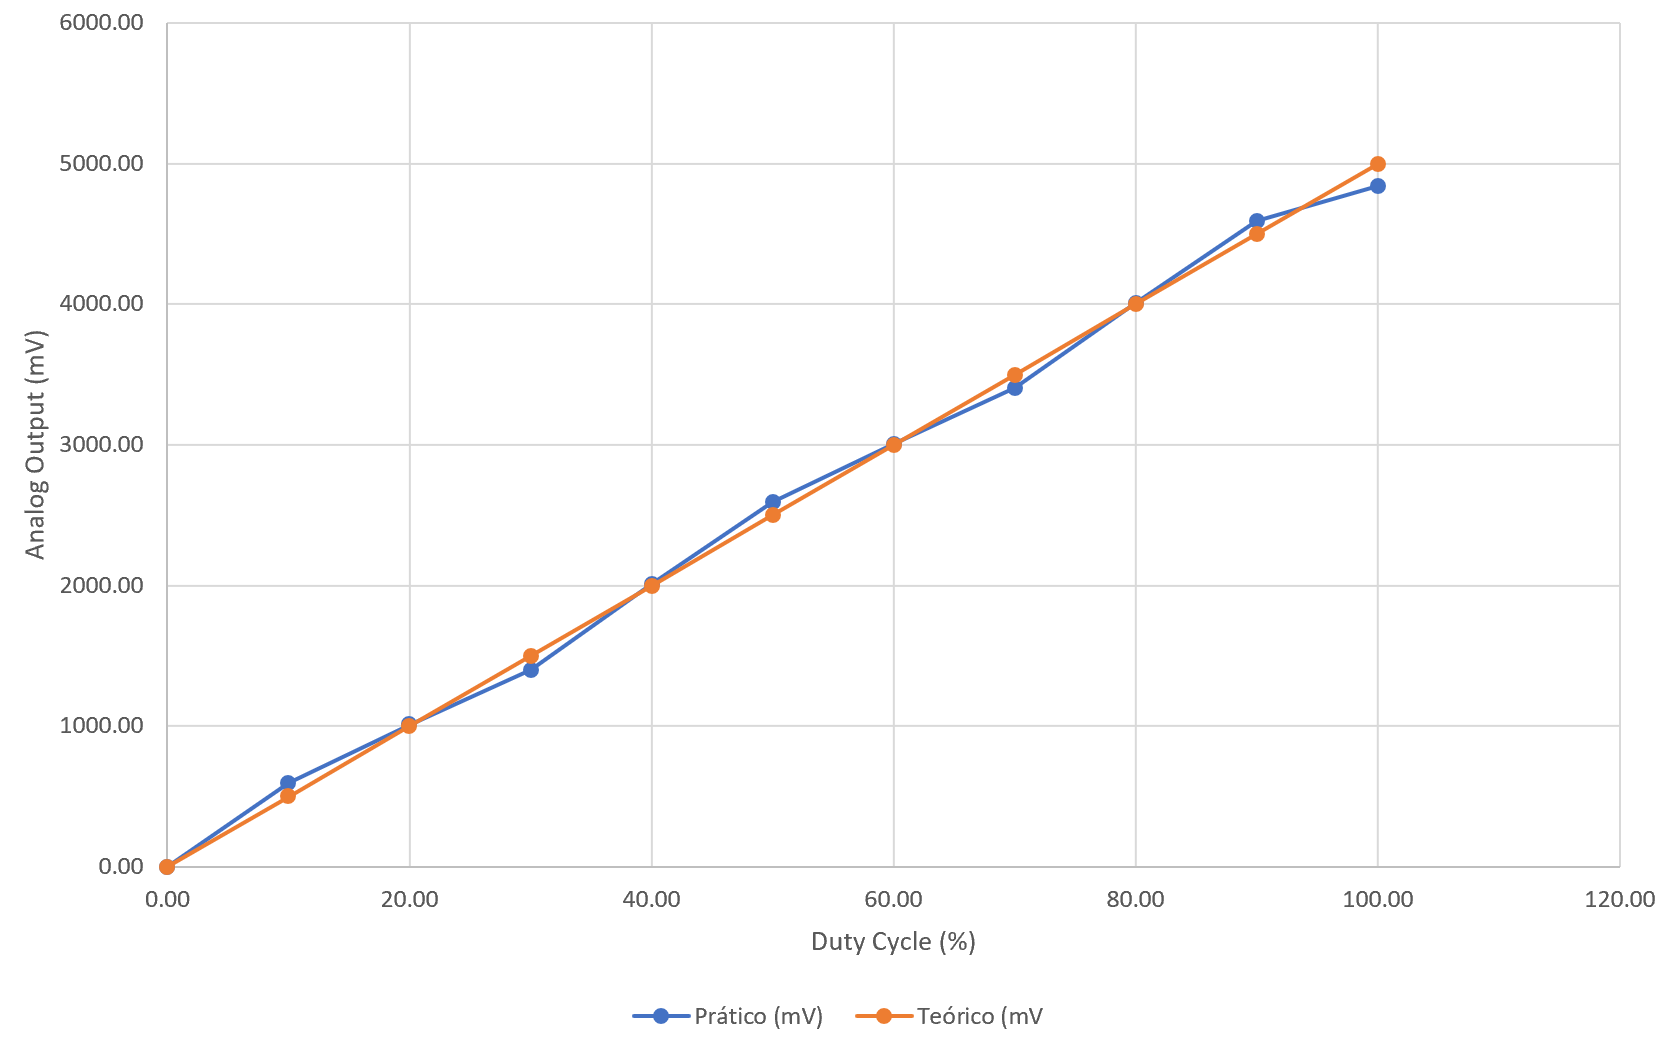
\includegraphics[width=1\textwidth]{figuras/fig-test-analog-voltage}
				\caption{Analog Output in Respect with Duty Cycle}
				\label{fig:test-analog-voltage}
		\end{figure}

		It is possible to see that the measured output was really faithful to the theoretically calculated output, the average error was just 3.35$\%$ which is pretty low. If we disconsider the measured values from 0$\%$ and 100$\%$ this erros falls to 1.58$\%$, probably this is related to the fact that 0$\%$ and 100$\%$ produces a theoretically output of 0V and 5V, which is respectively the negative and positive supply of the operational amplifier from the analog output circuit (check Section \ref{ssec:pwm-to-speed-reference-circuit}). Although the error for 0$\%$ and 100$\%$ is more than two times the error from the rest of the possible duty cycles, it still is quite small, and this happens because the chosen amplifier for the analog output circuit has rail-to-rail input/output.
		\par

		Different from the brake tests from Sections \ref{ssec:full-stop-test} and \ref{ssec:full-stop-test-results}, the frequency inverter was always on, the consequence of this is that the noise from the electric motor and the frequency inverter was always interfering with the CKP sensor signal. Figure \ref{fig:test-analog-rotation} shows the measured rotation in respect with the duty cycle.

		\begin{figure}[htbp]
				\centering
				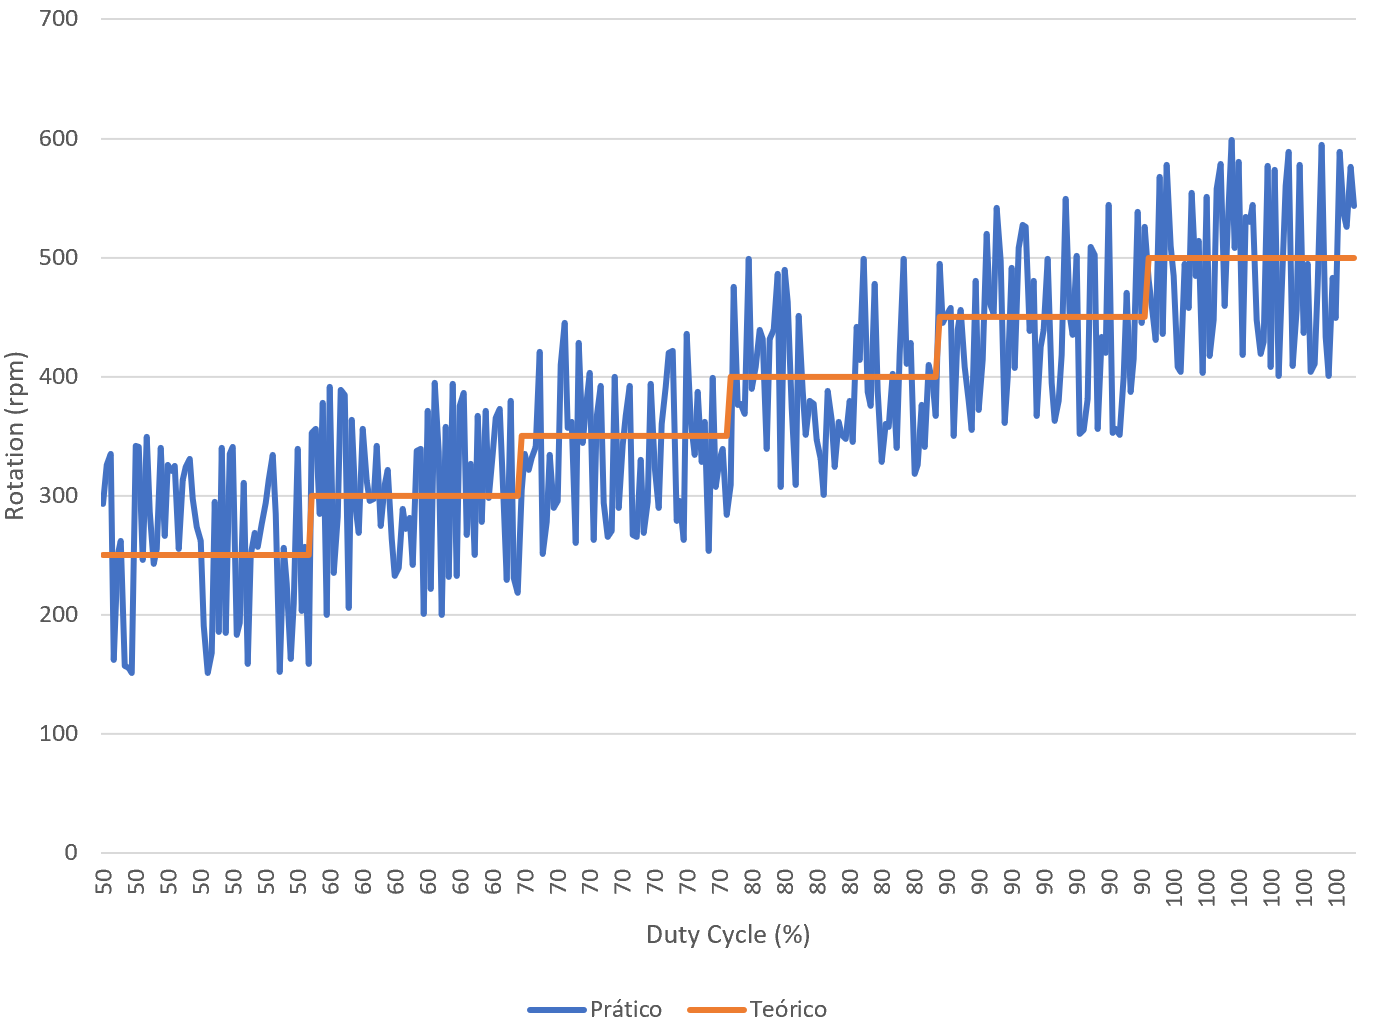
\includegraphics[width=1\textwidth]{figuras/fig-test-analog-rotation}
				\caption{Rotation in Respect with Duty Cycle}
				\label{fig:test-analog-rotation}
		\end{figure}

		The signal is extremely noisy, compared to the theoretical rotation. However, even with all that noise it is possible to see that the signal is varying within a range close to the desired rotation. Maybe with a more sophisticated software it would be possible to treat this signal better to achieve better results.